\documentclass[twoside]{book}

% Packages required by doxygen
\usepackage{fixltx2e}
\usepackage{calc}
\usepackage{doxygen}
\usepackage[export]{adjustbox} % also loads graphicx
\usepackage{graphicx}
\usepackage[utf8]{inputenc}
\usepackage{makeidx}
\usepackage{multicol}
\usepackage{multirow}
\PassOptionsToPackage{warn}{textcomp}
\usepackage{textcomp}
\usepackage[nointegrals]{wasysym}
\usepackage[table]{xcolor}

% Font selection
\usepackage[T1]{fontenc}
\usepackage[scaled=.90]{helvet}
\usepackage{courier}
\usepackage{amssymb}
\usepackage{sectsty}
\renewcommand{\familydefault}{\sfdefault}
\allsectionsfont{%
  \fontseries{bc}\selectfont%
  \color{darkgray}%
}
\renewcommand{\DoxyLabelFont}{%
  \fontseries{bc}\selectfont%
  \color{darkgray}%
}
\newcommand{\+}{\discretionary{\mbox{\scriptsize$\hookleftarrow$}}{}{}}

% Page & text layout
\usepackage{geometry}
\geometry{%
  a4paper,%
  top=2.5cm,%
  bottom=2.5cm,%
  left=2.5cm,%
  right=2.5cm%
}
\tolerance=750
\hfuzz=15pt
\hbadness=750
\setlength{\emergencystretch}{15pt}
\setlength{\parindent}{0cm}
\setlength{\parskip}{3ex plus 2ex minus 2ex}
\makeatletter
\renewcommand{\paragraph}{%
  \@startsection{paragraph}{4}{0ex}{-1.0ex}{1.0ex}{%
    \normalfont\normalsize\bfseries\SS@parafont%
  }%
}
\renewcommand{\subparagraph}{%
  \@startsection{subparagraph}{5}{0ex}{-1.0ex}{1.0ex}{%
    \normalfont\normalsize\bfseries\SS@subparafont%
  }%
}
\makeatother

% Headers & footers
\usepackage{fancyhdr}
\pagestyle{fancyplain}
\fancyhead[LE]{\fancyplain{}{\bfseries\thepage}}
\fancyhead[CE]{\fancyplain{}{}}
\fancyhead[RE]{\fancyplain{}{\bfseries\leftmark}}
\fancyhead[LO]{\fancyplain{}{\bfseries\rightmark}}
\fancyhead[CO]{\fancyplain{}{}}
\fancyhead[RO]{\fancyplain{}{\bfseries\thepage}}
\fancyfoot[LE]{\fancyplain{}{}}
\fancyfoot[CE]{\fancyplain{}{}}
\fancyfoot[RE]{\fancyplain{}{\bfseries\scriptsize Generated by Doxygen }}
\fancyfoot[LO]{\fancyplain{}{\bfseries\scriptsize Generated by Doxygen }}
\fancyfoot[CO]{\fancyplain{}{}}
\fancyfoot[RO]{\fancyplain{}{}}
\renewcommand{\footrulewidth}{0.4pt}
\renewcommand{\chaptermark}[1]{%
  \markboth{#1}{}%
}
\renewcommand{\sectionmark}[1]{%
  \markright{\thesection\ #1}%
}

% Indices & bibliography
\usepackage{natbib}
\usepackage[titles]{tocloft}
\setcounter{tocdepth}{3}
\setcounter{secnumdepth}{5}
\makeindex

% Packages requested by user
\usepackage{amsmath}

% Hyperlinks (required, but should be loaded last)
\usepackage{ifpdf}
\ifpdf
  \usepackage[pdftex,pagebackref=true]{hyperref}
\else
  \usepackage[ps2pdf,pagebackref=true]{hyperref}
\fi
\hypersetup{%
  colorlinks=true,%
  linkcolor=blue,%
  citecolor=blue,%
  unicode%
}

% Custom commands
\newcommand{\clearemptydoublepage}{%
  \newpage{\pagestyle{empty}\cleardoublepage}%
}

\usepackage{caption}
\captionsetup{labelsep=space,justification=centering,font={bf},singlelinecheck=off,skip=4pt,position=top}

%===== C O N T E N T S =====

\begin{document}

% Titlepage & ToC
\hypersetup{pageanchor=false,
             bookmarksnumbered=true,
             pdfencoding=unicode
            }
\pagenumbering{roman}
\begin{titlepage}
\vspace*{7cm}
\begin{center}%
{\Large Microphysics Scheme in C\+C\+PP }\\
\vspace*{1cm}
{\large Generated by Doxygen 1.8.11}\\
\end{center}
\end{titlepage}
\clearemptydoublepage
\tableofcontents
\clearemptydoublepage
\pagenumbering{arabic}
\hypersetup{pageanchor=true}

%--- Begin generated contents ---
\chapter{Grid-\/scale Condensation, Evaporation and Precipitation}
\label{index}\hypertarget{index}{}\hypertarget{index_Introduction}{}\section{Introduction}\label{index_Introduction}
Radiative process is one of the most complex and computational intensive part of all model physics. As an essential part of model physics, it directly and indirectly connects all physics processes with model dynamics, and regulates the overall earth-\/atmosphere energy exchanges and transformations. The radiation package in N\+E\+MS physics has standardized component modules. The schematic radiation module structure is shown in table 1.



Radiation parameterizations are intended to provide a fast and accurate method of determined the total radiative flux at any given location. These calculations provide both the total radiative flux at the ground surface, which is needed for the surface energy budget, and the vertical radiative flux divergence, which is used to calculate the radiative heating and cooling rates of a given atmospheric volume. The magnitude of the terms in the surface energy budget can set the stage for moist deep convection and are crucial to the formation of low-\/level clouds. In addition, the vertical radiative flux divergence can produce substantial cooling, particularly at the tops of clouds, which can have strong dynamic effect on cloud evolution.

The shortwave radiation parameterization is based on Chou and Suarez (1999) and was modified by Hou et al.(2002) for the G\+FS. It contains eight spectral bands in the ultraviolet and visible region and one spectral band in the near-\/infrared region. It includes absorption by ozone, water vapor,carbon dioxide, and oxygen. A random-\/maximum cloud overlapping is assumed for radiative transfer calculations in the operational G\+FS. Cloud optical depth is parameterized as a function of the predicted cloud condensate path and the effective radius of cloud particles ( $r_e$). Cloud particle single-\/scattering albedo and asymmetry factors are functions of $r_e$. For water droplets. $r_e$ is fixed at $10\mu m$ over the ocean, and specified as $r_e=min[max(5-0.25T_c , 5),10]\mu m$ over land, where $T_c$ is temperature in degrees Celsius. For ice particles, $r_e$ is an empirical function of ice water content and temperature that follows Heymsfield and Mc\+Farquhar (1996). The radiative effects of rain and snow are not included in the operational G\+FS, but the direct radiative effect of atmospheric aerosols is included. The surface albedo over land varies with the surface type, solar spectral band, and season, and is further adjusted by a solar zenith-\/angle-\/dependent factor for the direct solar beam. When the ground has snow cover the grid-\/mean surface albedo is first computed separately for snow-\/free and snow-\/covered areas, and then combined using a snow-\/cover fraction that depends on the surface roughness and snow depth. Snow albedo depends on the solar zenith angle (Briegleb 1992).

A major change was made in longwave radiation on 28 August 2003. The Geophysical Fluid Dynamics Laboratory (G\+F\+DL) model (Schwarzkopf and Fels 1991) was replaced by the Rapid Radiative Transfer Model (R\+R\+TM; Mlawer et al. 1997). The R\+R\+TM computes longwave absorption and emission by water vapor,carbon dioxide,ozone,cloud particles, and various trace gases including $N_2O$, $CH_4$, $O_2$,and four types of halocarbons\mbox{[}chlorofluorocarbons(\+C\+F\+Cs)\mbox{]}.Aerosol effects are not included.\+For consistency with the earlier G\+F\+DL module, no trace gases are included in the R\+R\+TM for the G\+FS forecasts. The R\+R\+TM uses a correlated-\/k distribution method and a transmittance lookup table that is linearly scaled by optical depth to achieve high accuracy and efficiency. The algorithm contains 140 unevenly distributed intervals in 16 spectral bands. It employs the Clough-\/\+Kneizys-\/\+Davies (C\+K\+D\+\_\+2.\+4) continuum model (Clough et al. 1992) to compute absorption by water vapor at the continuum band. Longwave cloud radiative properties external to the R\+R\+TM depend on cloud liquid/ice water path and the effective radius of ice particles and water droplets (Hu and Stamnes 1993; Ebert and Curry 1992).\hypertarget{index_mainpage-components}{}\section{Radiation Scheme Modules}\label{index_mainpage-components}
The following links take you to more information about each module.
\begin{DoxyItemize}
\item Driver Module\+: \hyperlink{namespacemodule__radiation__driver}{module\+\_\+radiation\+\_\+driver}
\item Shortwave(\+S\+W) Module\+: \hyperlink{namespacemodule__radsw__main}{module\+\_\+radsw\+\_\+main}
\item Longwave(\+L\+W) Module\+: \hyperlink{namespacemodule__radlw__main}{module\+\_\+radlw\+\_\+main}
\item Astronomy Module\+: \hyperlink{namespacemodule__radiation__astronomy}{module\+\_\+radiation\+\_\+astronomy}
\item Aerosol Module\+: \hyperlink{namespacemodule__radiation__aerosols}{module\+\_\+radiation\+\_\+aerosols}
\item Cloud Module\+: \hyperlink{namespacemodule__radiation__clouds}{module\+\_\+radiation\+\_\+clouds}
\item Surface Module\+: \hyperlink{namespacemodule__radiation__surface}{module\+\_\+radiation\+\_\+surface}
\item Gases Module\+: \hyperlink{namespacemodule__radiation__gases}{module\+\_\+radiation\+\_\+gases}
\end{DoxyItemize}\hypertarget{index_component}{}\section{Cloud Properties in Radiation}\label{index_component}
The cloud cover is calculated based on Xu and Randall (1996). \[ \sigma =RH^{k_{1}}\left[1-exp\left(-\frac{k_{2}q_{l}}{\left[\left(1-RH\right)q_{s}\right]^{k_{3}}}\right)\right] \] Where $RH$ is relative humidity, $q_{l}$ is the cloud condensate, $q_{s}$ is saturation specific humidity, $k_{1}(=0.25)$, $k_{2}(=100)$, $k_{3}(=0.49)$ are the empirical parameters. The cloud condensate is partitioned into cloud water and ice in radiation based on temperature. Cloud drop effective radius ranges 5-\/10 microns over land depending on temperature. Ice crystal radius is function of ice water content (Heymsfield and Mc\+Farquhar (1996)). Maximum-\/randomly cloud overlapping is used in both long-\/wave radiation and short-\/wave radiation. Convective clouds are not considered in radiation.\hypertarget{index_component}{}\section{Cloud Properties in Radiation}\label{index_component}

\begin{DoxyItemize}
\item Updated and optimized R\+R\+T\+MG + Neural Net Emulator option
\item Higher frequency of radiation calls (possibly every time step with NN)
\item Uncorrelated cloud overlap \& inhomogeneous water/ice clouds with rain/snow
\item Updated C\+O2 with vertically varying profile
\item Observed estimate of trace gases -\/ prescribed global mean climatology
\item Mean solar constant of 1361 $W/m^2$ (with 11 year solar cycle -\/ Van Den Dool)
\item G\+O\+C\+A\+RT interactive aerosol model, updated with vertical profile
\item Land albedo using M\+O\+D\+IS retrieval based monthly data
\item Ocean albedo based on salinity, surface wind and Cosz
\item Spectrally varing emissivity
\end{DoxyItemize}\hypertarget{index_References}{}\section{References}\label{index_References}
Barker, H. W., et al., 2003\+: Assessing 1D atmospheric solar radiative transfer models\+: interpretation and handling of unresolved clouds. J. Clim., 16, 2676-\/2699.

Briegleb, B. P., 1992\+: Delta-\/\+Eddington approximation for solar radiation in the N\+C\+AR community climate model. J. Geophys. Res., 97, 7603-\/7612.

Briegleb, B. P., P. Minnus, V. Ramanathan, and E. Harrison, 1986\+: Comparison of regional clear-\/sky albedo inferred from satellite observations and model computations. J. Clim. and Appl. Meteo., 25, 214-\/226.

Chin, M., R. B. Rood, S-\/J. Lin, J-\/F. Mller, and A. M. Thompson, 2000\+: Atmospheric sulfur cycle simulated in the global model G\+O\+C\+A\+RT\+: Model description and global properties. J. Geophys. Res., 105, 24671-\/24687.

Chou, M. D., M. J. Suarez, C. H. Ho, M. M. H. Yan, and K. T. Lee, 1998\+: Parameterizations for cloud overlapping and shortwave single scattering properties for use in general circulation and cloud ensemble models. J. Clim., 11, 202-\/214.

Clough, S. A., and M. J. Iacono, 1995\+: Line-\/by-\/line calculation of atmospheric fluxes and cooling rates\+: 2. Application to carbon dioxide, ozone, methane, nitrous oxide and the halocarbons. J. Geophys. Res.\+100, 16519-\/16535.

Clough, S. A., M. W. Shephard, E. J. Mlawer, J. S. delamere, M. J. Iacono, K. Cady-\/\+Pereira, S. Boukabara, and P. D. Brown, 2005\+: Atmospheric radiative transfer modeling\+: a summary of the A\+ER codes, J. Quant. Spectrosc. Radiat. Transfer, 91, 233-\/244.

Coakley, J. A., R. D. Cess, and F. B. Yurevich, 1983\+: The effect of tropospheric aerosols on the earth\textquotesingle{}s radiation budget\+: a parameterization for climate models. J. Atmos. Sci., 42, 1408-\/1429.

Fels, S. B., and M.\+D. Schwarzkopf, 1975\+: The simplified exchange approximation\+: A new method for radiative transfer calculations. J. Atmos. Sci., 337, 2265-\/2297.

Frohlich, C. and G. E. Shaw, 1980\+: New determination of Rayleigh scattering in the terrestrial atmosphere. Appl. Opt., 14, 1773-\/1775.

Fu, Q., 1996\+: An accurate parameterization of the solar radiative properties of cirrus clouds for climate models. J. Clim., 9, 2058-\/2082.

Fu, Q., P. Yang, and W.\+B. Sun, 1998\+: An accurate parameterization of the infrared radiative properties of cirrus clouds for climate models. J. Clim., 11, 2223-\/2237.

Hess, M., P. Koepke, and I. Schult, 1998\+: Optical properties of aerosols and clouds\+: The software package O\+P\+AC. Bull. Am. Meteor. Soc., 79, 831-\/844.

Heymsfield, A. J., and G. M. Mc\+Farquhar, 1996\+: High albedos of cirrus in the tropical Pacific warm pool. J. Atmos. Sci., 53, 2424-\/2451.

Hou, Y-\/T., S. Moorthi, K. Campana, 2002\+: Parameterization of solar radiation transfer in the N\+C\+EP Models. N\+C\+EP Office Note 441, 46pp.

Hu, Y. X., and K. Stamnes. 1993\+: An accurate parameterization of the radiative properties of water clouds suitable for use in climate models. J. Clim., 6, 728-\/742.

Kiehl, J. T., J. J. Hack, G. B. Bonan, B. A. Boville, D. L. Williamson, and P. J. Rasch, 1998\+: The national center for atmospheric research community climate model C\+C\+M3. J. Clim., 11, 1131-\/1149.

Matthews, E., 1985\+: Atlas of Archived Vegetation, Land Use, and Seasonal Albedo Data Sets., N\+A\+SA Technical Memorandum 86199, Goddard Institute for Space Studies, New York.

Mlawer, E. J., S. J. Taubman, P. D. Brown, M. J. Iacono, and S. A. Clough, 1997\+: Radiative transfer for inhomogenerous atmospheres\+: R\+R\+TM, a validated correlated-\/k model for the longwave. J. Geophys. Res., 102, 16663-\/16682.

Oreopoulos, L. and Barker, H. W., 1999\+: Accounting for subgrid-\/scale cloud variability in a multi-\/layer, 1D solar radiative transfer algorithm. Q. J. R. Meteorol. Soc., 125, 301-\/330.

Pincus, R., Barker, H. W. and Morcrette, J.-\/J., 2003\+: A fast, flexible, approximate technique of computing radiative transfer for inhomogeneous clouds. J. Geophys. Res., 108, 4376, doi\+: 10.\+1029/2002\+J\+D003322.

Roberts, R. E., J. A. Selby, and L. M. Biberman, 1976\+: Infrared continuum absorption by atmospheric water vapor in the 8-\/12 micron window. Appl. Optics., 15, 2085-\/2090.

Rodgers, C.\+D., 1968\+: Some extension and applications of the new random model for molecular band transmission. Quart. J. Roy. Meteor. Soc., 94,99-\/102.

Sato, M., J. E. Hansen, M. P. Mc\+Cormick, and J. B. Pollack, 1993\+: Stratospheric aerosol optical depth, 1850-\/1990. J. Geophys. Res., 98, 22987-\/22994.

Slingo, A., 1989\+: A G\+CM parameterization for the shortwave radiative properties pf water clouds. J. Atmos. Sci., 46, 1419-\/1427.

Schwarzkopf, M.\+D., and S. B. Fels, 1985\+: Improvements to the algorithm for computing C\+O2 transmissivities and cooling rates. J. Geophys. Res., 90, 10541-\/10550.

Schwarzkopf, M.\+D., and S. B. Fels, 1991\+: The simplified exchange method revisited\+: An accurate, rapid method for computation of infrared cooling rates and fluxes. J. Geophys. Res., 96, 9075-\/9096.

Staylor, W. F. and A. C. Wilbur, 1990\+: Global surface albedos estimated from E\+R\+BE data. Preprints of the Seventh Conference on Atmospheric Radiation, San Francisco CA, American Meteorological Society, 231-\/236.

Stephens, G. L., 1984\+: The parameterization of radiation for numerical weather prediction and climate models. Mon. Wea. Rev., 112, 826-\/867.

Zdunkowski, W. G., Welsch, R. M., and Korb, G. J., 1980\+: An investigation of the structure of typical 2-\/stream methods for the calculation of solar fluxes and heating rates in clouds. Contrib. Atms. Phys., 53, 215-\/238. 
\chapter{Todo List}
\label{todo}
\hypertarget{todo}{}

\begin{DoxyRefList}
\item[\label{todo__todo000001}%
\hypertarget{todo__todo000001}{}%
Subprogram \hyperlink{namespacemodule__radiation__clouds_a1953118ed22c3b6f8d94ef231b47a08b}{module\+\_\+radiation\+\_\+clouds\+:\+:progcld3} ]document the difference with progcld1 
\end{DoxyRefList}
\chapter{File Index}
\section{File List}
Here is a list of all files with brief descriptions\+:\begin{DoxyCompactList}
\item\contentsline{section}{\hyperlink{grrad_8f}{grrad.\+f} }{\pageref{grrad_8f}}{}
\item\contentsline{section}{\hyperlink{module__bfmicrophysics_8f}{module\+\_\+bfmicrophysics.\+f} }{\pageref{module__bfmicrophysics_8f}}{}
\item\contentsline{section}{\hyperlink{physcons_8f}{physcons.\+f} }{\pageref{physcons_8f}}{}
\item\contentsline{section}{\hyperlink{physparam_8f}{physparam.\+f} }{\pageref{physparam_8f}}{}
\item\contentsline{section}{\hyperlink{rad__initialize_8f}{rad\+\_\+initialize.\+f} }{\pageref{rad__initialize_8f}}{}
\item\contentsline{section}{\hyperlink{radiation__aerosols_8f}{radiation\+\_\+aerosols.\+f} }{\pageref{radiation__aerosols_8f}}{}
\item\contentsline{section}{\hyperlink{radiation__astronomy_8f}{radiation\+\_\+astronomy.\+f} }{\pageref{radiation__astronomy_8f}}{}
\item\contentsline{section}{\hyperlink{radiation__clouds_8f}{radiation\+\_\+clouds.\+f} }{\pageref{radiation__clouds_8f}}{}
\item\contentsline{section}{\hyperlink{radiation__gases_8f}{radiation\+\_\+gases.\+f} }{\pageref{radiation__gases_8f}}{}
\item\contentsline{section}{\hyperlink{radiation__surface_8f}{radiation\+\_\+surface.\+f} }{\pageref{radiation__surface_8f}}{}
\item\contentsline{section}{\hyperlink{radlw__datatb_8f}{radlw\+\_\+datatb.\+f} }{\pageref{radlw__datatb_8f}}{}
\item\contentsline{section}{\hyperlink{radlw__main_8f}{radlw\+\_\+main.\+f} }{\pageref{radlw__main_8f}}{}
\item\contentsline{section}{\hyperlink{radlw__param_8f}{radlw\+\_\+param.\+f} }{\pageref{radlw__param_8f}}{}
\item\contentsline{section}{\hyperlink{radsw__datatb_8f}{radsw\+\_\+datatb.\+f} }{\pageref{radsw__datatb_8f}}{}
\item\contentsline{section}{\hyperlink{radsw__main_8f}{radsw\+\_\+main.\+f} }{\pageref{radsw__main_8f}}{}
\item\contentsline{section}{\hyperlink{radsw__param_8f}{radsw\+\_\+param.\+f} }{\pageref{radsw__param_8f}}{}
\item\contentsline{section}{\hyperlink{schematic___rad__mod_8png}{schematic\+\_\+\+Rad\+\_\+mod.\+png} }{\pageref{schematic___rad__mod_8png}}{}
\end{DoxyCompactList}

\chapter{File Documentation}
\hypertarget{calpreciptype_8f}{}\section{calpreciptype.\+f File Reference}
\label{calpreciptype_8f}\index{calpreciptype.\+f@{calpreciptype.\+f}}
\subsection*{Functions/\+Subroutines}
\begin{DoxyCompactItemize}
\item 
subroutine \hyperlink{calpreciptype_8f_ace3ba03fce51ab8bd25977ff03a99c1d}{calwxt} (lm, lp1, t, q, pmid, pint,                                                                                                                                                   d608, rog, epsq, zint, iwx, twet)
\begin{DoxyCompactList}\small\item\em This subroutine computes precipitation type using a decision tree approach that uses variables such as integrated wet bulb temp below freezing and lowest layer temperature. \end{DoxyCompactList}\item 
subroutine \hyperlink{calpreciptype_8f_a1359538b0437522a5643286d47cb956d}{calwxt\+\_\+ramer} (lm, lp1, t, q, pmid, rh, td, pint, ptyp)
\begin{DoxyCompactList}\small\item\em This subroutine is written and provided by Jim Ramer at N\+O\+A\+A/\+F\+SL. \end{DoxyCompactList}\item 
real function \hyperlink{calpreciptype_8f_a761529912bd612dc070ad13eb14de778}{xmytw} (t, td, p)
\item 
subroutine \hyperlink{calpreciptype_8f_aeb6ff6c9bfe0ac826d6b0e28c0592223}{calwxt\+\_\+bourg} (lm, lp1, rn, g, t, q, pmid, pint, zint, ptype)
\begin{DoxyCompactList}\small\item\em This subrtouien computes precipitation type using a decision tree approach that uses the so-\/called \char`\"{}energy method\char`\"{} of Bourgouin of A\+ES (Canada) 1992. \end{DoxyCompactList}\item 
subroutine \hyperlink{calpreciptype_8f_aea4e1369bc96598ada546c7aa96988cd}{calwxt\+\_\+revised} (lm, lp1, t, q, pmid, pint,                                                                                                                                                               d608, rog, epsq, zint, twet, iwx)
\begin{DoxyCompactList}\small\item\em This subroutine computes precipitation type using a decision tree approach that uses variables such as integrated wet bulb temp below freezing and lowest layer temperature. \end{DoxyCompactList}\item 
subroutine \hyperlink{calpreciptype_8f_a84b16fee5df628928b15bfbde86ee0ca}{calwxt\+\_\+explicit} (lm, tskin, sr, f\+\_\+rimef, iwx)
\begin{DoxyCompactList}\small\item\em The subroutine computes precipitation type using explicit fields from the model microphysics. \end{DoxyCompactList}\item 
subroutine \hyperlink{calpreciptype_8f_aa8cf475c2ada385565809d05de8fb215}{calwxt\+\_\+dominant} (nalg, rain, freezr, sleet, snow,                                                                                                           domr, domzr, domip, doms)
\begin{DoxyCompactList}\small\item\em This subroutine takes the precip type solutions from different algorithms and sums them up to give a domain type. \end{DoxyCompactList}\end{DoxyCompactItemize}
{\bf }\par
\begin{DoxyCompactItemize}
\item 
subroutine \hyperlink{calpreciptype_8f_a8a471b8f23f55928b69814c887ec925a}{calpreciptype} (kdt, nrcm, im, ix, lm, lp1, randomno,                                                                                                                                           xlat, xlon,                                                                                                                                                                                                                               gt0, gq0, prsl, prsi, prec,                                                                                                                                                                           phii, n3dfercld, tskin, sr, phy\+\_\+f3d,                                                                                                                                       domr, domzr, domip, doms)
\begin{DoxyCompactList}\small\item\em This subroutine computes precipitation type. It is adopted from post but was made into column to used by G\+FS model. \end{DoxyCompactList}\end{DoxyCompactItemize}



\subsection{Function/\+Subroutine Documentation}
\index{calpreciptype.\+f@{calpreciptype.\+f}!calpreciptype@{calpreciptype}}
\index{calpreciptype@{calpreciptype}!calpreciptype.\+f@{calpreciptype.\+f}}
\subsubsection[{\texorpdfstring{calpreciptype(kdt, nrcm, im, ix, lm, lp1, randomno,                                                                                                                                           xlat, xlon,                                                                                                                                                                                                                               gt0, gq0, prsl, prsi, prec,                                                                                                                                                                           phii, n3dfercld, tskin, sr, phy\+\_\+f3d,                                                                                                                                       domr, domzr, domip, doms)}{calpreciptype(kdt, nrcm, im, ix, lm, lp1, randomno,                                                                                                                                           xlat, xlon,                                                                                                                                                                                                                               gt0, gq0, prsl, prsi, prec,                                                                                                                                                                           phii, n3dfercld, tskin, sr, phy_f3d,                                                                                                                                       domr, domzr, domip, doms)}}]{\setlength{\rightskip}{0pt plus 5cm}subroutine calpreciptype (
\begin{DoxyParamCaption}
\item[{integer, intent(in)}]{kdt, }
\item[{integer, intent(in)}]{nrcm, }
\item[{integer, intent(in)}]{im, }
\item[{integer, intent(in)}]{ix, }
\item[{integer, intent(in)}]{lm, }
\item[{integer, intent(in)}]{lp1, }
\item[{real, dimension(ix,nrcm), intent(in)}]{randomno, }
\item[{real, dimension(im), intent(in)}]{xlat, }
\item[{real, dimension(im), intent(in)}]{xlon, }
\item[{real(kind=kind\+\_\+phys), dimension(ix,lm), intent(in)}]{gt0, }
\item[{real(kind=kind\+\_\+phys), dimension(ix,lm), intent(in)}]{gq0, }
\item[{real(kind=kind\+\_\+phys), dimension(ix,lm), intent(in)}]{prsl, }
\item[{real(kind=kind\+\_\+phys), dimension(ix,lp1), intent(in)}]{prsi, }
\item[{real(kind=kind\+\_\+phys), dimension(im), intent(in)}]{prec, }
\item[{real(kind=kind\+\_\+phys), dimension(ix,lp1), intent(in)}]{phii, }
\item[{integer, intent(in)}]{n3dfercld, }
\item[{real(kind=kind\+\_\+phys), dimension(im), intent(in)}]{tskin, }
\item[{real(kind=kind\+\_\+phys), dimension(im), intent(in)}]{sr, }
\item[{real(kind=kind\+\_\+phys), dimension(ix,lm), intent(in)}]{phy\+\_\+f3d, }
\item[{real(kind=kind\+\_\+phys), dimension(im), intent(out)}]{domr, }
\item[{real(kind=kind\+\_\+phys), dimension(im), intent(out)}]{domzr, }
\item[{real(kind=kind\+\_\+phys), dimension(im), intent(out)}]{domip, }
\item[{real(kind=kind\+\_\+phys), dimension(im), intent(out)}]{doms}
\end{DoxyParamCaption}
)}\hypertarget{calpreciptype_8f_a8a471b8f23f55928b69814c887ec925a}{}\label{calpreciptype_8f_a8a471b8f23f55928b69814c887ec925a}

\begin{DoxyParams}[1]{Parameters}
\mbox{\tt in}  & {\em kdt} & integer, 1, number of the current time step \\
\hline
\mbox{\tt in}  & {\em nrcm} & integer, 1, second dimension for the random number array rann \\
\hline
\mbox{\tt in}  & {\em im} & integer, 1, horizontal number of used pts \\
\hline
\mbox{\tt in}  & {\em ix} & integer, 1, horizontal dimension \\
\hline
\mbox{\tt in}  & {\em lm} & integer, 1, vertical layer dimension \\
\hline
\mbox{\tt in}  & {\em lp1} & integer, 1, lm+1 \\
\hline
\mbox{\tt in}  & {\em randomno} & real,(ix,nrcm),random number array (0-\/1) \\
\hline
\mbox{\tt in}  & {\em xlat} & real,(im),latitude (radian) \\
\hline
\mbox{\tt in}  & {\em xlon} & real,(im),longitude (radian) \\
\hline
\mbox{\tt in}  & {\em gt0} & real,(ix,lm), updated temperature \\
\hline
\mbox{\tt in}  & {\em gq0} & real,(ix,lm), updated tracers\\
\hline
\end{DoxyParams}
\begin{DoxyRefDesc}{Todo}
\item[\hyperlink{todo__todo000001}{Todo}]dimension of gq0 should be (ix,lm,ntrac)? \end{DoxyRefDesc}

\begin{DoxyParams}[1]{Parameters}
\mbox{\tt in}  & {\em prsl} & real,(ix,lm), mean layer pressure \\
\hline
\mbox{\tt in}  & {\em prsi} & real,(ix,lp1), pressure at layer interfaces \\
\hline
\mbox{\tt in}  & {\em prec} & real,(im), total rain at this time step (rain) \\
\hline
\mbox{\tt in}  & {\em phii} & real,(ix,lp1), interface geopotential $(m^2/s^2)$ \\
\hline
\mbox{\tt in}  & {\em n3dfercld} & integer,1,number of 3D arrays needed for microphysics(num\+\_\+p3d) \\
\hline
\mbox{\tt in}  & {\em tskin} & real,(im), ground surface temperature in K (tsea) \\
\hline
\mbox{\tt in}  & {\em sr} & real,(im), ratio of snow to total precipitation \\
\hline
\mbox{\tt in}  & {\em phy\+\_\+f3d} & real,(ix,lm), 3d arrays saved for restart \\
\hline
\mbox{\tt out}  & {\em domr} & real,(im), dominant precip type for rain \\
\hline
\mbox{\tt out}  & {\em domzr} & real,(im), dominant precip type for freezing rain \\
\hline
\mbox{\tt out}  & {\em domip} & real,(im), dominant precip type for sleet \\
\hline
\mbox{\tt out}  & {\em doms} & real,(im), dominant precip type for snow \\
\hline
\end{DoxyParams}
\hypertarget{gscond_8f_general}{}\subsection{General Algorithm}\label{gscond_8f_general}

\begin{DoxyEnumerate}
\item Compute wet bulb temperature
\item call \hyperlink{calpreciptype_8f_ace3ba03fce51ab8bd25977ff03a99c1d}{calwxt()} to compute instantaneous precipitation type.
\item For Ramer algorithm, call \hyperlink{calpreciptype_8f_a1359538b0437522a5643286d47cb956d}{calwxt\+\_\+ramer()}
\item For Bourgouin algorithm, call \hyperlink{calpreciptype_8f_aeb6ff6c9bfe0ac826d6b0e28c0592223}{calwxt\+\_\+bourg()}
\item For revised N\+C\+EP algorithm, call \hyperlink{calpreciptype_8f_aea4e1369bc96598ada546c7aa96988cd}{calwxt\+\_\+revised()}
\item For explicit algorithm(n3dfercld=3,ferrier\textquotesingle{}s scheme), call \hyperlink{calpreciptype_8f_a84b16fee5df628928b15bfbde86ee0ca}{calwxt\+\_\+explicit()}
\item call \hyperlink{calpreciptype_8f_aa8cf475c2ada385565809d05de8fb215}{calwxt\+\_\+dominant()} to compute dominant precip type 
\end{DoxyEnumerate}

Definition at line 33 of file calpreciptype.\+f.



References calwxt(), calwxt\+\_\+bourg(), calwxt\+\_\+dominant(), calwxt\+\_\+explicit(), calwxt\+\_\+ramer(), and calwxt\+\_\+revised().



Referenced by gbphys().



Here is the call graph for this function\+:\nopagebreak
\begin{figure}[H]
\begin{center}
\leavevmode
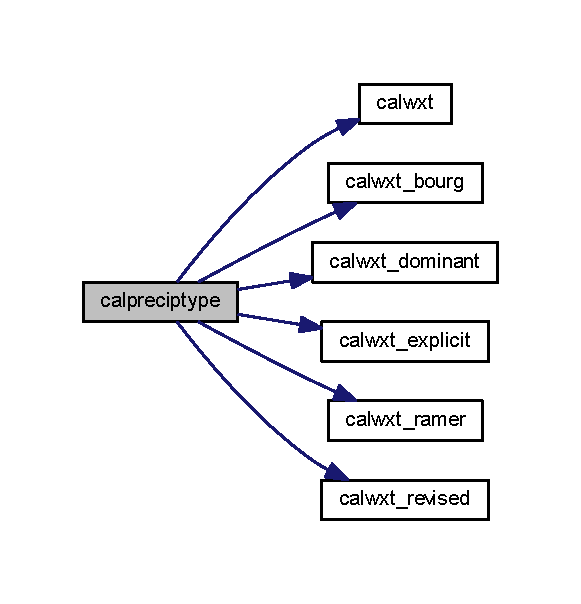
\includegraphics[width=279pt]{calpreciptype_8f_a8a471b8f23f55928b69814c887ec925a_cgraph}
\end{center}
\end{figure}




Here is the caller graph for this function\+:\nopagebreak
\begin{figure}[H]
\begin{center}
\leavevmode
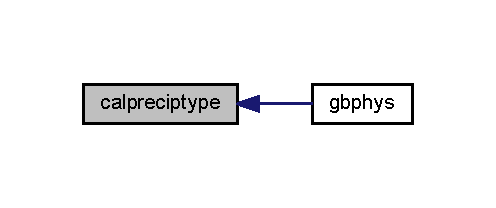
\includegraphics[width=238pt]{calpreciptype_8f_a8a471b8f23f55928b69814c887ec925a_icgraph}
\end{center}
\end{figure}


\index{calpreciptype.\+f@{calpreciptype.\+f}!calwxt@{calwxt}}
\index{calwxt@{calwxt}!calpreciptype.\+f@{calpreciptype.\+f}}
\subsubsection[{\texorpdfstring{calwxt(lm, lp1, t, q, pmid, pint,                                                                                                                                                   d608, rog, epsq, zint, iwx, twet)}{calwxt(lm, lp1, t, q, pmid, pint,                                                                                                                                                   d608, rog, epsq, zint, iwx, twet)}}]{\setlength{\rightskip}{0pt plus 5cm}subroutine calwxt (
\begin{DoxyParamCaption}
\item[{integer, intent(in)}]{lm, }
\item[{integer, intent(in)}]{lp1, }
\item[{real, dimension(lm), intent(in)}]{t, }
\item[{real, dimension(lm), intent(in)}]{q, }
\item[{real, dimension(lm), intent(in)}]{pmid, }
\item[{real, dimension(lp1), intent(in)}]{pint, }
\item[{real, intent(in)}]{d608, }
\item[{real, intent(in)}]{rog, }
\item[{real, intent(in)}]{epsq, }
\item[{real, dimension(lp1), intent(in)}]{zint, }
\item[{integer, intent(out)}]{iwx, }
\item[{real, dimension(lm), intent(in)}]{twet}
\end{DoxyParamCaption}
)}\hypertarget{calpreciptype_8f_ace3ba03fce51ab8bd25977ff03a99c1d}{}\label{calpreciptype_8f_ace3ba03fce51ab8bd25977ff03a99c1d}

\begin{DoxyItemize}
\item see baldwin and contorno 
\end{DoxyItemize}

Definition at line 256 of file calpreciptype.\+f.



Referenced by calpreciptype().



Here is the caller graph for this function\+:\nopagebreak
\begin{figure}[H]
\begin{center}
\leavevmode
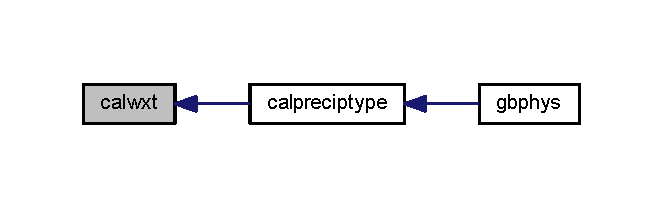
\includegraphics[width=318pt]{calpreciptype_8f_ace3ba03fce51ab8bd25977ff03a99c1d_icgraph}
\end{center}
\end{figure}


\index{calpreciptype.\+f@{calpreciptype.\+f}!calwxt\+\_\+bourg@{calwxt\+\_\+bourg}}
\index{calwxt\+\_\+bourg@{calwxt\+\_\+bourg}!calpreciptype.\+f@{calpreciptype.\+f}}
\subsubsection[{\texorpdfstring{calwxt\+\_\+bourg(lm, lp1, rn, g, t, q, pmid, pint, zint, ptype)}{calwxt_bourg(lm, lp1, rn, g, t, q, pmid, pint, zint, ptype)}}]{\setlength{\rightskip}{0pt plus 5cm}subroutine calwxt\+\_\+bourg (
\begin{DoxyParamCaption}
\item[{integer, intent(in)}]{lm, }
\item[{integer, intent(in)}]{lp1, }
\item[{real, dimension(2), intent(in)}]{rn, }
\item[{real, intent(in)}]{g, }
\item[{real, dimension(lm), intent(in)}]{t, }
\item[{real, dimension(lm), intent(in)}]{q, }
\item[{real, dimension(lm), intent(in)}]{pmid, }
\item[{real, dimension(lp1), intent(in)}]{pint, }
\item[{real, dimension(lp1), intent(in)}]{zint, }
\item[{integer, intent(out)}]{ptype}
\end{DoxyParamCaption}
)}\hypertarget{calpreciptype_8f_aeb6ff6c9bfe0ac826d6b0e28c0592223}{}\label{calpreciptype_8f_aeb6ff6c9bfe0ac826d6b0e28c0592223}


Definition at line 908 of file calpreciptype.\+f.



Referenced by calpreciptype().



Here is the caller graph for this function\+:\nopagebreak
\begin{figure}[H]
\begin{center}
\leavevmode
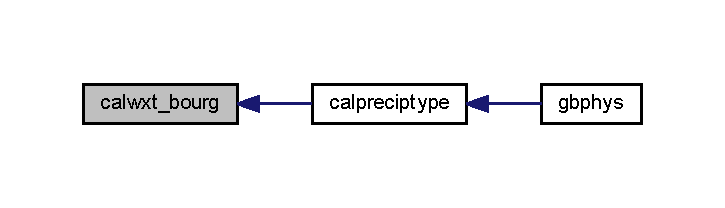
\includegraphics[width=348pt]{calpreciptype_8f_aeb6ff6c9bfe0ac826d6b0e28c0592223_icgraph}
\end{center}
\end{figure}


\index{calpreciptype.\+f@{calpreciptype.\+f}!calwxt\+\_\+dominant@{calwxt\+\_\+dominant}}
\index{calwxt\+\_\+dominant@{calwxt\+\_\+dominant}!calpreciptype.\+f@{calpreciptype.\+f}}
\subsubsection[{\texorpdfstring{calwxt\+\_\+dominant(nalg, rain, freezr, sleet, snow,                                                                                                           domr, domzr, domip, doms)}{calwxt_dominant(nalg, rain, freezr, sleet, snow,                                                                                                           domr, domzr, domip, doms)}}]{\setlength{\rightskip}{0pt plus 5cm}subroutine calwxt\+\_\+dominant (
\begin{DoxyParamCaption}
\item[{integer, intent(in)}]{nalg, }
\item[{integer, dimension(nalg), intent(in)}]{rain, }
\item[{integer, dimension(nalg), intent(in)}]{freezr, }
\item[{integer, dimension(nalg), intent(in)}]{sleet, }
\item[{integer, dimension(nalg), intent(in)}]{snow, }
\item[{real, intent(out)}]{domr, }
\item[{real, intent(out)}]{domzr, }
\item[{real, intent(out)}]{domip, }
\item[{real, intent(out)}]{doms}
\end{DoxyParamCaption}
)}\hypertarget{calpreciptype_8f_aa8cf475c2ada385565809d05de8fb215}{}\label{calpreciptype_8f_aa8cf475c2ada385565809d05de8fb215}


Definition at line 1400 of file calpreciptype.\+f.



Referenced by calpreciptype().



Here is the caller graph for this function\+:\nopagebreak
\begin{figure}[H]
\begin{center}
\leavevmode
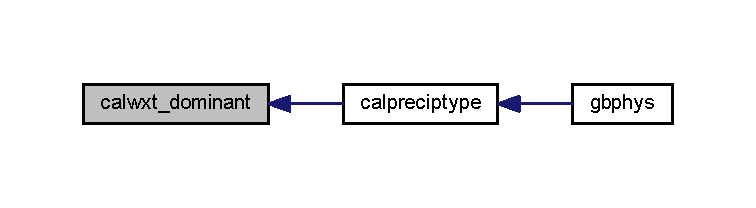
\includegraphics[width=350pt]{calpreciptype_8f_aa8cf475c2ada385565809d05de8fb215_icgraph}
\end{center}
\end{figure}


\index{calpreciptype.\+f@{calpreciptype.\+f}!calwxt\+\_\+explicit@{calwxt\+\_\+explicit}}
\index{calwxt\+\_\+explicit@{calwxt\+\_\+explicit}!calpreciptype.\+f@{calpreciptype.\+f}}
\subsubsection[{\texorpdfstring{calwxt\+\_\+explicit(lm, tskin, sr, f\+\_\+rimef, iwx)}{calwxt_explicit(lm, tskin, sr, f_rimef, iwx)}}]{\setlength{\rightskip}{0pt plus 5cm}subroutine calwxt\+\_\+explicit (
\begin{DoxyParamCaption}
\item[{integer, intent(in)}]{lm, }
\item[{real, intent(in)}]{tskin, }
\item[{real, intent(in)}]{sr, }
\item[{real, dimension(lm), intent(in)}]{f\+\_\+rimef, }
\item[{integer, intent(out)}]{iwx}
\end{DoxyParamCaption}
)}\hypertarget{calpreciptype_8f_a84b16fee5df628928b15bfbde86ee0ca}{}\label{calpreciptype_8f_a84b16fee5df628928b15bfbde86ee0ca}


Definition at line 1337 of file calpreciptype.\+f.



Referenced by calpreciptype().



Here is the caller graph for this function\+:\nopagebreak
\begin{figure}[H]
\begin{center}
\leavevmode
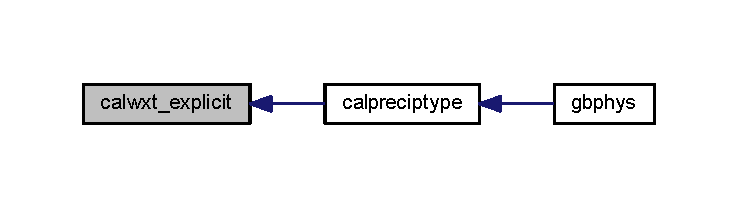
\includegraphics[width=350pt]{calpreciptype_8f_a84b16fee5df628928b15bfbde86ee0ca_icgraph}
\end{center}
\end{figure}


\index{calpreciptype.\+f@{calpreciptype.\+f}!calwxt\+\_\+ramer@{calwxt\+\_\+ramer}}
\index{calwxt\+\_\+ramer@{calwxt\+\_\+ramer}!calpreciptype.\+f@{calpreciptype.\+f}}
\subsubsection[{\texorpdfstring{calwxt\+\_\+ramer(lm, lp1, t, q, pmid, rh, td, pint, ptyp)}{calwxt_ramer(lm, lp1, t, q, pmid, rh, td, pint, ptyp)}}]{\setlength{\rightskip}{0pt plus 5cm}subroutine calwxt\+\_\+ramer (
\begin{DoxyParamCaption}
\item[{integer, intent(in)}]{lm, }
\item[{integer, intent(in)}]{lp1, }
\item[{real, dimension(lm), intent(in)}]{t, }
\item[{real, dimension(lm), intent(in)}]{q, }
\item[{real, dimension(lm), intent(in)}]{pmid, }
\item[{real, dimension(lm), intent(in)}]{rh, }
\item[{real, dimension(lm), intent(in)}]{td, }
\item[{real, dimension(lp1), intent(in)}]{pint, }
\item[{integer, intent(out)}]{ptyp}
\end{DoxyParamCaption}
)}\hypertarget{calpreciptype_8f_a1359538b0437522a5643286d47cb956d}{}\label{calpreciptype_8f_a1359538b0437522a5643286d47cb956d}

\begin{DoxyItemize}
\item Ramer J, 1993\+: An expirical technique for diagnosing precipitation type from model output. preprints, 5th conf. on aviation weather systems, vienna, va, Amer. Meteor. Soc., 227-\/230. 
\end{DoxyItemize}

Definition at line 509 of file calpreciptype.\+f.



Referenced by calpreciptype().



Here is the caller graph for this function\+:\nopagebreak
\begin{figure}[H]
\begin{center}
\leavevmode
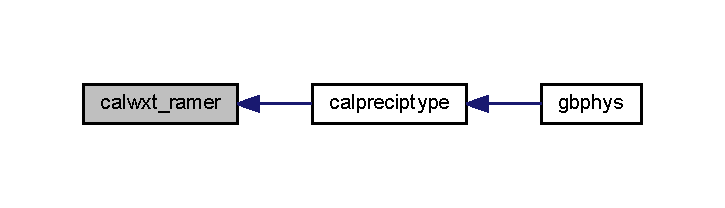
\includegraphics[width=348pt]{calpreciptype_8f_a1359538b0437522a5643286d47cb956d_icgraph}
\end{center}
\end{figure}


\index{calpreciptype.\+f@{calpreciptype.\+f}!calwxt\+\_\+revised@{calwxt\+\_\+revised}}
\index{calwxt\+\_\+revised@{calwxt\+\_\+revised}!calpreciptype.\+f@{calpreciptype.\+f}}
\subsubsection[{\texorpdfstring{calwxt\+\_\+revised(lm, lp1, t, q, pmid, pint,                                                                                                                                                               d608, rog, epsq, zint, twet, iwx)}{calwxt_revised(lm, lp1, t, q, pmid, pint,                                                                                                                                                               d608, rog, epsq, zint, twet, iwx)}}]{\setlength{\rightskip}{0pt plus 5cm}subroutine calwxt\+\_\+revised (
\begin{DoxyParamCaption}
\item[{integer, intent(in)}]{lm, }
\item[{integer, intent(in)}]{lp1, }
\item[{real, dimension(lm), intent(in)}]{t, }
\item[{real, dimension(lm), intent(in)}]{q, }
\item[{real, dimension(lm), intent(in)}]{pmid, }
\item[{real, dimension(lp1), intent(in)}]{pint, }
\item[{real, intent(in)}]{d608, }
\item[{real, intent(in)}]{rog, }
\item[{real, intent(in)}]{epsq, }
\item[{real, dimension(lp1), intent(in)}]{zint, }
\item[{real, dimension(lm), intent(in)}]{twet, }
\item[{integer, intent(out)}]{iwx}
\end{DoxyParamCaption}
)}\hypertarget{calpreciptype_8f_aea4e1369bc96598ada546c7aa96988cd}{}\label{calpreciptype_8f_aea4e1369bc96598ada546c7aa96988cd}

\begin{DoxyItemize}
\item see baldwin and contorno preprint from 13th weather analysis and forecasting conference for more details (or baldwin et al, 10th N\+WP conference preprint)
\item since the original version of the algorithm has a high bias for freezing rain and sleet, the goal is to balance that bias with a version more likely to predict snow 
\end{DoxyItemize}

Definition at line 1080 of file calpreciptype.\+f.



Referenced by calpreciptype().



Here is the caller graph for this function\+:\nopagebreak
\begin{figure}[H]
\begin{center}
\leavevmode
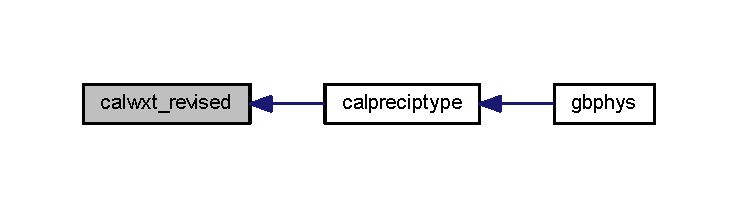
\includegraphics[width=350pt]{calpreciptype_8f_aea4e1369bc96598ada546c7aa96988cd_icgraph}
\end{center}
\end{figure}


\index{calpreciptype.\+f@{calpreciptype.\+f}!xmytw@{xmytw}}
\index{xmytw@{xmytw}!calpreciptype.\+f@{calpreciptype.\+f}}
\subsubsection[{\texorpdfstring{xmytw(t, td, p)}{xmytw(t, td, p)}}]{\setlength{\rightskip}{0pt plus 5cm}real function xmytw (
\begin{DoxyParamCaption}
\item[{real}]{t, }
\item[{real}]{td, }
\item[{real}]{p}
\end{DoxyParamCaption}
)}\hypertarget{calpreciptype_8f_a761529912bd612dc070ad13eb14de778}{}\label{calpreciptype_8f_a761529912bd612dc070ad13eb14de778}


Definition at line 786 of file calpreciptype.\+f.


\hypertarget{gbphys_8f}{}\section{gbphys.\+f File Reference}
\label{gbphys_8f}\index{gbphys.\+f@{gbphys.\+f}}
\subsection*{Functions/\+Subroutines}
\begin{DoxyCompactItemize}
\item 
subroutine \hyperlink{gbphys_8f_a34cd2db09b580c23df51c96d5905a805}{gbphys}                                                                                               
\end{DoxyCompactItemize}


\subsection{Function/\+Subroutine Documentation}
\index{gbphys.\+f@{gbphys.\+f}!gbphys@{gbphys}}
\index{gbphys@{gbphys}!gbphys.\+f@{gbphys.\+f}}
\subsubsection[{\texorpdfstring{gbphys                                                                                              }{gbphys                                                                                              }}]{\setlength{\rightskip}{0pt plus 5cm}subroutine gbphys (
\begin{DoxyParamCaption}
{}
\end{DoxyParamCaption}
)}\hypertarget{gbphys_8f_a34cd2db09b580c23df51c96d5905a805}{}\label{gbphys_8f_a34cd2db09b580c23df51c96d5905a805}


Definition at line 469 of file gbphys.\+f.



References calpreciptype(), gscond(), gscondp(), gsmdrive(), precpd(), precpd\+\_\+shoc(), and precpdp().



Here is the call graph for this function\+:
\nopagebreak
\begin{figure}[H]
\begin{center}
\leavevmode
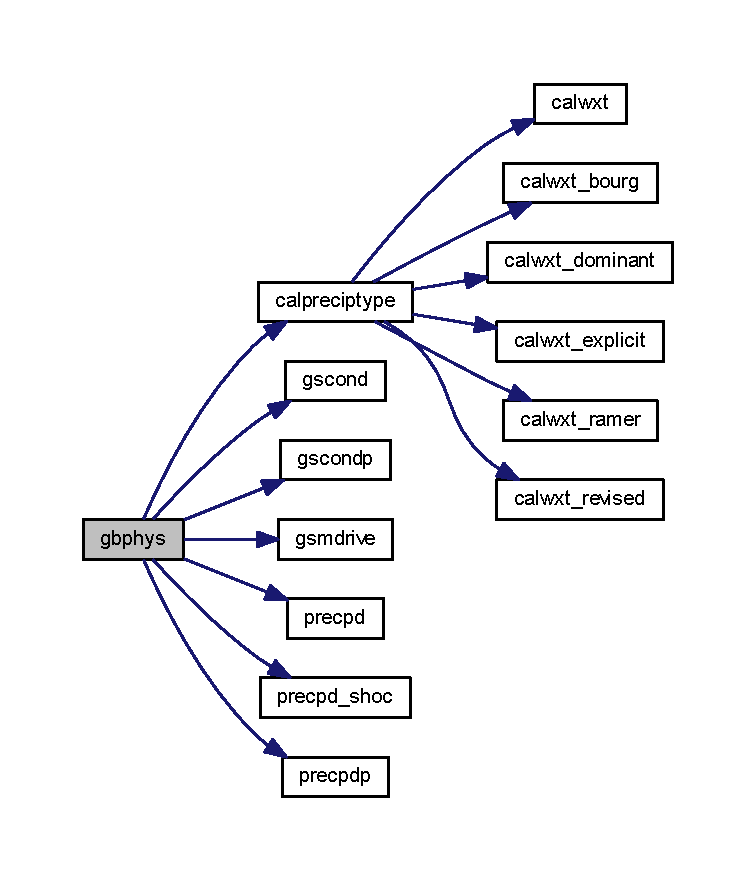
\includegraphics[width=350pt]{gbphys_8f_a34cd2db09b580c23df51c96d5905a805_cgraph}
\end{center}
\end{figure}



\hypertarget{gscond_8f}{}\section{gscond.\+f File Reference}
\label{gscond_8f}\index{gscond.\+f@{gscond.\+f}}
\subsection*{Functions/\+Subroutines}
{\bf }\par
\begin{DoxyCompactItemize}
\item 
subroutine \hyperlink{gscond_8f_a02cb3895f68b86a4b7e259c8c098ecc1}{gscond} (im, ix, km, dt, dtf, prsl, ps, q, cwm, t                                                           ,                                                               tp, qp, psp, tp1, qp1, psp1, u, lprnt, ipr)
\begin{DoxyCompactList}\small\item\em This subroutine is for grid-\/scale condensation\&evaporation for the mrf model at N\+C\+EP. \end{DoxyCompactList}\end{DoxyCompactItemize}



\subsection{Function/\+Subroutine Documentation}
\index{gscond.\+f@{gscond.\+f}!gscond@{gscond}}
\index{gscond@{gscond}!gscond.\+f@{gscond.\+f}}
\subsubsection[{\texorpdfstring{gscond(im, ix, km, dt, dtf, prsl, ps, q, cwm, t                                                           ,                                                               tp, qp, psp, tp1, qp1, psp1, u, lprnt, ipr)}{gscond(im, ix, km, dt, dtf, prsl, ps, q, cwm, t                                                           ,                                                               tp, qp, psp, tp1, qp1, psp1, u, lprnt, ipr)}}]{\setlength{\rightskip}{0pt plus 5cm}subroutine gscond (
\begin{DoxyParamCaption}
\item[{integer}]{im, }
\item[{integer}]{ix, }
\item[{integer}]{km, }
\item[{}]{dt, }
\item[{}]{dtf, }
\item[{}]{prsl, }
\item[{}]{ps, }
\item[{real (kind=kind\+\_\+phys), dimension(ix,km)}]{q, }
\item[{real (kind=kind\+\_\+phys), dimension(ix,km)}]{cwm, }
\item[{real (kind=kind\+\_\+phys), dimension(ix,km)}]{t, }
\item[{}]{tp, }
\item[{}]{qp, }
\item[{}]{psp, }
\item[{}]{tp1, }
\item[{}]{qp1, }
\item[{}]{psp1, }
\item[{real (kind=kind\+\_\+phys), dimension(im,km)}]{u, }
\item[{logical}]{lprnt, }
\item[{integer}]{ipr}
\end{DoxyParamCaption}
)}\hypertarget{gscond_8f_a02cb3895f68b86a4b7e259c8c098ecc1}{}\label{gscond_8f_a02cb3895f68b86a4b7e259c8c098ecc1}

\begin{DoxyParams}[1]{Parameters}
\mbox{\tt in}  & {\em ix,im} & integer, 1, horizontal dimension and num of used pts \\
\hline
\mbox{\tt in}  & {\em km} & integer, 1, vertical layer dimension \\
\hline
\mbox{\tt in}  & {\em dt} & real, 1, physics time step in seconds \\
\hline
\mbox{\tt in}  & {\em dtf} & real, 1, dynamics time step in seconds \\
\hline
\mbox{\tt in}  & {\em prsl} & real, (ix,km), mean layer pressure \\
\hline
\mbox{\tt in}  & {\em ps} & real, (im), surface pressure (Pa) \\
\hline
\mbox{\tt in,out}  & {\em q} & real, (ix,km), updated tracers (gq0(\+:,\+:,1)) \\
\hline
\mbox{\tt in,out}  & {\em cwm} & real, (ix,km), updated tracers (gq0(\+:,\+:,ntcw)) \\
\hline
\mbox{\tt in,out}  & {\em t} & real, (ix,km), updated temperature \\
\hline
\mbox{\tt in,out}  & {\em tp} & real, (ix,km), see phy\+\_\+f3d(\+:,\+:,1) \\
\hline
\mbox{\tt in,out}  & {\em qp} & real, (ix,km), see phy\+\_\+f3d(\+:,\+:,2) \\
\hline
\mbox{\tt in,out}  & {\em psp} & real, (im), see phy\+\_\+f2d(\+:,1) \\
\hline
\mbox{\tt in,out}  & {\em tp1} & real, (ix,km), see phy\+\_\+f3d(\+:,\+:,3) \\
\hline
\mbox{\tt in,out}  & {\em qp1} & real, (ix,km), see phy\+\_\+f3d(\+:,\+:,4) \\
\hline
\mbox{\tt in,out}  & {\em psp1} & real, (im), see phy\+\_\+f2d(\+:,2) \\
\hline
\mbox{\tt in}  & {\em u} & real, (im,km), the critical value of relative humidity for large-\/scale condensation \\
\hline
\mbox{\tt in}  & {\em lprnt} & logical print flag \\
\hline
\mbox{\tt in}  & {\em ipr} & integer, 1, check print point for debugging \\
\hline
\end{DoxyParams}
\hypertarget{gscond_8f_general}{}\subsection{General Algorithm}\label{gscond_8f_general}

\begin{DoxyEnumerate}
\item Compute ice-\/water id number IW.
\begin{DoxyItemize}
\item see Table 2 in Zhao and Carr (1997)\+: The distinction between cloud water and cloud ice is made by the cloud identification number IW, which is zero for cloud water and unity for cloud ice.
\item All clouds are defined to consist of liquid water below the freezing level ( $T>0^oC$) and of ice particles above the $T=-15^oC$ level.
\item In the temperature region between these two, clouds may be either cloud water or cloud ice. If there are cloud ice particles above this point at the previous or current time step, or if the cloud at this point at the previous time step consists of ice particles, then the cloud substance at this point should also be ice particles because of the cloud seeding effect and the cloud memory of its content.
\item Otherwise, all clouds in this region are considered to contain supercooled cloud water.
\end{DoxyItemize}
\item Condensation and evaporation of cloud
\begin{DoxyItemize}
\item Compute at,aq and ap, which are the changes in t,q and p caused by all the processes except grid-\/scale condensation and evaporation.
\item Compute the satuation specific humidity and the relative humidity
\item According to Sunqvist et al. (1989), cloud fraction $b$ at a grid point can be estimated from relative humidity using the equation \[ b=1-\left ( \frac{f_{s}-f}{f_{s}-f_{0}} \right )^{1/2} \] for $f>f_{0}$, and $ccr=0$ for $f<f_{0}$. where $f_{s}=1.0$ is the relative humidity in a cloud region. $f_{0}$ is the critical value of relative humidity for large-\/scale condensation. ~\newline
 Since both temperature and moisture may vary at scales smaller than model grid scale, it is possible for condensation to occur before the grid-\/average relative humidity reaches 100\%. Therefore $f_{0}$ needs to be less than 1.\+0 to account for the subgrid-\/scale variation of temperature and moisture fields.
\item If cloud cover $\leq $ cclimitm then evaporate any existing cloud condensate ( $E_{c}$) ~\newline
 If $q_{0}$ represents the specific humidity at relative humidity $f_{0}$, then \[ q_{0}=f_{0}q_{s} \] ~\newline
 if the cloud water/ice at this point is enough to be evaporated until $f_{0}$ is reached, then the evaporation rate $E_{c}$, if we assume that the evaporation process occurs in one time step, is determined by \[ E_{c}=\frac{q_{0}-q}{\triangle t} \] ~\newline
 using $q_{0}=f_{0}q_{s}$ and the equation $q=fq_{s}$, $E_{c}$ then becomes \[ E_{c}=\frac{q_{s}}{\triangle t}(f_{0}-f) \] where $\triangle t$ is the time step for precipitation calculation in the model.\+It is a simplified version of a higher-\/order cloud evaporation algorithm (Rutledge and Hobbs 1983).
\item If cloud over $>$ cclimit, condense water vapor in to cloud condensate ( $C_{g}$) ~\newline
 Following Sundqvist et al.(1989), the grid-\/scale condensation rate is solving ( $C_{g}$) from Eqs (6) and (7) with equations $q=fq_{s}$, $q_{s}=\epsilon e_{s}/p$, and the Clausius-\/\+Clapeyron equation $de_{s}/dT=\epsilon Le_{s}/RT^{2}$,where $q_{s}$ is the saturation specific humidity, $e_{s}$ is the saturation vapor pressure, $R$ is the specific gas constant for dry air, $P$ is the pressure, $f$ is the relative humidity, and $\epsilon=0.622$. The expression for $C_{g}$ has the form \[ C_{g}=\frac{M-q_{s}f_{t}}{1+(f\epsilon L^{2}q_{s}/RC_{p}T^{2})}+E_{c} \] where \[ M=A_{q}-\frac{f\epsilon Lq_{s}}{RT^{2}}A_{t}+\frac{fq_{s}\partial p}{p\partial t} \] To close the system, an equation for relative humidity tendency $f_{t}$ was derived by Sundqvist et al. (1989) using the hypothesis that the quantity $M+E_{c}$ is divided into one part, $bM$,which condenses in the already cloudy portion of a grid square, and another part, $(1-b)M+E_{c}$,which is used to increase the relative humidity of the cloud-\/free portion and to increase the cloudiness in the square. The equation is written as \[ f_{t}=\frac{2(1-b)(f_{s}-f_{0})[(1-b)M+E_{c}]}{2q_{s}(1-b)(f_{s}-f_{0})+m/b} \]
\item Check \& correct if over condensation occurs
\item Update of t, q and cwm (see Eqs(6),(7) in Zhao and Carr (1997)) \[ cwm=cwm+(C_{g}-E_{c})\times dt \] \[ q=q-(C_{g}-E_{c})\times dt \] \[ t=t+\frac{L}{C_{p}}(C_{g}-E_{c})\times dt \] ~\newline
 where $L$ is the latent heat of condensation/deposition, $C_{p}$ is the specific heat of air at constant pressure.
\end{DoxyItemize}
\item Store $t$, $q$, $ps$ for next time step 
\end{DoxyEnumerate}

Definition at line 27 of file gscond.\+f.



Referenced by gbphys().



Here is the caller graph for this function\+:
\nopagebreak
\begin{figure}[H]
\begin{center}
\leavevmode
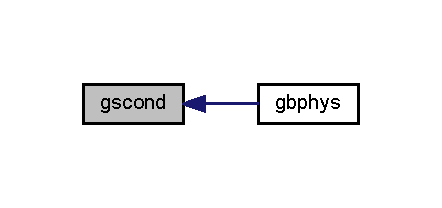
\includegraphics[width=212pt]{gscond_8f_a02cb3895f68b86a4b7e259c8c098ecc1_icgraph}
\end{center}
\end{figure}



\hypertarget{gscondp_8f}{}\section{gscondp.\+f File Reference}
\label{gscondp_8f}\index{gscondp.\+f@{gscondp.\+f}}
\subsection*{Functions/\+Subroutines}
\begin{DoxyCompactItemize}
\item 
subroutine \hyperlink{gscondp_8f_a604b82ae595aa7783efaa32cfde39e98}{gscondp} (im, ix, km, dt, dtf, prsl, ps, q, cwm, t               ,                                                               tp, qp, psp, tp1, qp1, psp1                   ,u, deltaq, sup, lprnt, ipr, kdt)
\end{DoxyCompactItemize}


\subsection{Function/\+Subroutine Documentation}
\index{gscondp.\+f@{gscondp.\+f}!gscondp@{gscondp}}
\index{gscondp@{gscondp}!gscondp.\+f@{gscondp.\+f}}
\subsubsection[{\texorpdfstring{gscondp(im, ix, km, dt, dtf, prsl, ps, q, cwm, t               ,                                                               tp, qp, psp, tp1, qp1, psp1                   ,u, deltaq, sup, lprnt, ipr, kdt)}{gscondp(im, ix, km, dt, dtf, prsl, ps, q, cwm, t               ,                                                               tp, qp, psp, tp1, qp1, psp1                   ,u, deltaq, sup, lprnt, ipr, kdt)}}]{\setlength{\rightskip}{0pt plus 5cm}subroutine gscondp (
\begin{DoxyParamCaption}
\item[{integer}]{im, }
\item[{integer}]{ix, }
\item[{integer}]{km, }
\item[{real (kind=kind\+\_\+phys)}]{dt, }
\item[{real (kind=kind\+\_\+phys)}]{dtf, }
\item[{real (kind=kind\+\_\+phys), dimension(ix,km)}]{prsl, }
\item[{real (kind=kind\+\_\+phys), dimension(im)}]{ps, }
\item[{real (kind=kind\+\_\+phys), dimension(ix,km)}]{q, }
\item[{real (kind=kind\+\_\+phys), dimension(ix,km)}]{cwm, }
\item[{real (kind=kind\+\_\+phys), dimension(ix,km)}]{t, }
\item[{real (kind=kind\+\_\+phys), dimension(ix,km)}]{tp, }
\item[{real (kind=kind\+\_\+phys), dimension(ix,km)}]{qp, }
\item[{real (kind=kind\+\_\+phys), dimension(im)}]{psp, }
\item[{real (kind=kind\+\_\+phys), dimension(ix,km)}]{tp1, }
\item[{real (kind=kind\+\_\+phys), dimension(ix,km)}]{qp1, }
\item[{real (kind=kind\+\_\+phys), dimension(im)}]{psp1, }
\item[{real (kind=kind\+\_\+phys), dimension(im,km)}]{u, }
\item[{real (kind=kind\+\_\+phys), dimension(ix,km)}]{deltaq, }
\item[{real (kind=kind\+\_\+phys), intent(in)}]{sup, }
\item[{logical}]{lprnt, }
\item[{integer}]{ipr, }
\item[{integer}]{kdt}
\end{DoxyParamCaption}
)}\hypertarget{gscondp_8f_a604b82ae595aa7783efaa32cfde39e98}{}\label{gscondp_8f_a604b82ae595aa7783efaa32cfde39e98}


Definition at line 4 of file gscondp.\+f.



Referenced by gbphys().



Here is the caller graph for this function\+:
\nopagebreak
\begin{figure}[H]
\begin{center}
\leavevmode
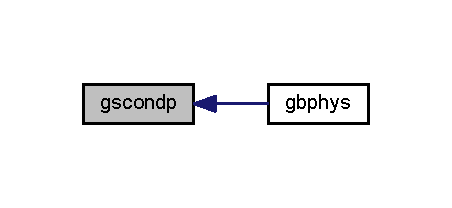
\includegraphics[width=217pt]{gscondp_8f_a604b82ae595aa7783efaa32cfde39e98_icgraph}
\end{center}
\end{figure}



\hypertarget{gsmddrive_8f}{}\section{gsmddrive.\+f File Reference}
\label{gsmddrive_8f}\index{gsmddrive.\+f@{gsmddrive.\+f}}
\subsection*{Functions/\+Subroutines}
\begin{DoxyCompactItemize}
\item 
subroutine \hyperlink{gsmddrive_8f_afa4aee02bd0f01dde988f4b8621466a7}{gsmdrive} (im, ix, lm, dt, grav, hvap, hsub, cp,                                                                                               me, lprnt, ipr,                                                                                               prsl, del, rhc, xncw, flgmin,                                                                                               tin, qin, ccin,                                                                                               f\+\_\+ice, f\+\_\+rain, f\+\_\+rimef, aprec, sr)
\item 
subroutine \hyperlink{gsmddrive_8f_a545ecb105d9ac23b8913dfbf8655d0a0}{micro\+\_\+init} (len1, len2, num\+\_\+p3d, len4, phy\+\_\+f3d,                                                                                                                                                           DT, F\+H\+O\+UR, me, first)
\item 
subroutine \hyperlink{gsmddrive_8f_ae360e5361d937fd832e108b923f60532}{init\+\_\+micro} (D\+TP, len1, len2, num\+\_\+p3d, len4, phy\+\_\+f3d, fhour, me)
\end{DoxyCompactItemize}


\subsection{Function/\+Subroutine Documentation}
\index{gsmddrive.\+f@{gsmddrive.\+f}!gsmdrive@{gsmdrive}}
\index{gsmdrive@{gsmdrive}!gsmddrive.\+f@{gsmddrive.\+f}}
\subsubsection[{\texorpdfstring{gsmdrive(im, ix, lm, dt, grav, hvap, hsub, cp,                                                                                               me, lprnt, ipr,                                                                                               prsl, del, rhc, xncw, flgmin,                                                                                               tin, qin, ccin,                                                                                               f\+\_\+ice, f\+\_\+rain, f\+\_\+rimef, aprec, sr)}{gsmdrive(im, ix, lm, dt, grav, hvap, hsub, cp,                                                                                               me, lprnt, ipr,                                                                                               prsl, del, rhc, xncw, flgmin,                                                                                               tin, qin, ccin,                                                                                               f_ice, f_rain, f_rimef, aprec, sr)}}]{\setlength{\rightskip}{0pt plus 5cm}subroutine gsmdrive (
\begin{DoxyParamCaption}
\item[{integer}]{im, }
\item[{integer}]{ix, }
\item[{integer}]{lm, }
\item[{real (kind=kind\+\_\+phys)}]{dt, }
\item[{real (kind=kind\+\_\+phys)}]{grav, }
\item[{real (kind=kind\+\_\+phys)}]{hvap, }
\item[{real (kind=kind\+\_\+phys)}]{hsub, }
\item[{real (kind=kind\+\_\+phys)}]{cp, }
\item[{integer}]{me, }
\item[{logical}]{lprnt, }
\item[{integer}]{ipr, }
\item[{real (kind=kind\+\_\+phys), dimension(ix,lm)}]{prsl, }
\item[{real (kind=kind\+\_\+phys), dimension(ix,lm)}]{del, }
\item[{real (kind=kind\+\_\+phys), dimension(im,lm)}]{rhc, }
\item[{real (kind=kind\+\_\+phys), dimension(im)}]{xncw, }
\item[{real (kind=kind\+\_\+phys), dimension(im)}]{flgmin, }
\item[{real (kind=kind\+\_\+phys), dimension(ix,lm)}]{tin, }
\item[{real (kind=kind\+\_\+phys), dimension(ix,lm)}]{qin, }
\item[{real (kind=kind\+\_\+phys), dimension(ix,lm)}]{ccin, }
\item[{real (kind=kind\+\_\+phys), dimension(ix,lm)}]{f\+\_\+ice, }
\item[{real (kind=kind\+\_\+phys), dimension(ix,lm)}]{f\+\_\+rain, }
\item[{real (kind=kind\+\_\+phys), dimension(ix,lm)}]{f\+\_\+rimef, }
\item[{real (kind=kind\+\_\+phys), dimension(im)}]{aprec, }
\item[{real (kind=kind\+\_\+phys), dimension(im)}]{sr}
\end{DoxyParamCaption}
)}\hypertarget{gsmddrive_8f_afa4aee02bd0f01dde988f4b8621466a7}{}\label{gsmddrive_8f_afa4aee02bd0f01dde988f4b8621466a7}


Definition at line 16 of file gsmddrive.\+f.



Referenced by gbphys().



Here is the caller graph for this function\+:\nopagebreak
\begin{figure}[H]
\begin{center}
\leavevmode
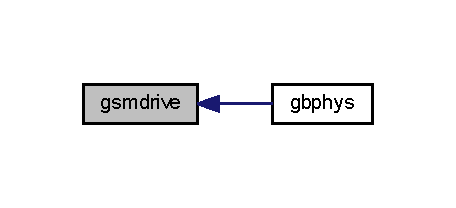
\includegraphics[width=219pt]{gsmddrive_8f_afa4aee02bd0f01dde988f4b8621466a7_icgraph}
\end{center}
\end{figure}


\index{gsmddrive.\+f@{gsmddrive.\+f}!init\+\_\+micro@{init\+\_\+micro}}
\index{init\+\_\+micro@{init\+\_\+micro}!gsmddrive.\+f@{gsmddrive.\+f}}
\subsubsection[{\texorpdfstring{init\+\_\+micro(\+D\+T\+P, len1, len2, num\+\_\+p3d, len4, phy\+\_\+f3d, fhour, me)}{init_micro(DTP, len1, len2, num_p3d, len4, phy_f3d, fhour, me)}}]{\setlength{\rightskip}{0pt plus 5cm}subroutine init\+\_\+micro (
\begin{DoxyParamCaption}
\item[{real (kind=kind\+\_\+phys)}]{D\+TP, }
\item[{integer}]{len1, }
\item[{integer}]{len2, }
\item[{integer}]{num\+\_\+p3d, }
\item[{integer}]{len4, }
\item[{real (kind=kind\+\_\+phys), dimension(len1,len2,num\+\_\+p3d,len4)}]{phy\+\_\+f3d, }
\item[{real (kind=kind\+\_\+phys)}]{fhour, }
\item[{integer}]{me}
\end{DoxyParamCaption}
)}\hypertarget{gsmddrive_8f_ae360e5361d937fd832e108b923f60532}{}\label{gsmddrive_8f_ae360e5361d937fd832e108b923f60532}


Definition at line 458 of file gsmddrive.\+f.



References micro\+\_\+init().



Here is the call graph for this function\+:\nopagebreak
\begin{figure}[H]
\begin{center}
\leavevmode
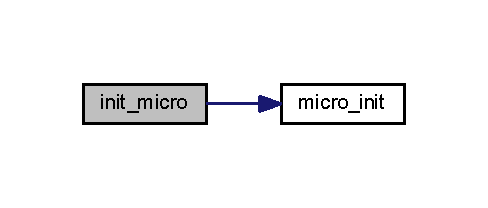
\includegraphics[width=234pt]{gsmddrive_8f_ae360e5361d937fd832e108b923f60532_cgraph}
\end{center}
\end{figure}


\index{gsmddrive.\+f@{gsmddrive.\+f}!micro\+\_\+init@{micro\+\_\+init}}
\index{micro\+\_\+init@{micro\+\_\+init}!gsmddrive.\+f@{gsmddrive.\+f}}
\subsubsection[{\texorpdfstring{micro\+\_\+init(len1, len2, num\+\_\+p3d, len4, phy\+\_\+f3d,                                                                                                                                                           D\+T, F\+H\+O\+U\+R, me, first)}{micro_init(len1, len2, num_p3d, len4, phy_f3d,                                                                                                                                                           DT, FHOUR, me, first)}}]{\setlength{\rightskip}{0pt plus 5cm}subroutine micro\+\_\+init (
\begin{DoxyParamCaption}
\item[{integer}]{len1, }
\item[{integer}]{len2, }
\item[{integer}]{num\+\_\+p3d, }
\item[{integer}]{len4, }
\item[{real (kind=kind\+\_\+phys), dimension(len1,len2,num\+\_\+p3d,len4)}]{phy\+\_\+f3d, }
\item[{real (kind=kind\+\_\+phys)}]{DT, }
\item[{real (kind=kind\+\_\+phys)}]{F\+H\+O\+UR, }
\item[{integer}]{me, }
\item[{logical}]{first}
\end{DoxyParamCaption}
)}\hypertarget{gsmddrive_8f_a545ecb105d9ac23b8913dfbf8655d0a0}{}\label{gsmddrive_8f_a545ecb105d9ac23b8913dfbf8655d0a0}


Definition at line 436 of file gsmddrive.\+f.



Referenced by init\+\_\+micro().



Here is the caller graph for this function\+:\nopagebreak
\begin{figure}[H]
\begin{center}
\leavevmode
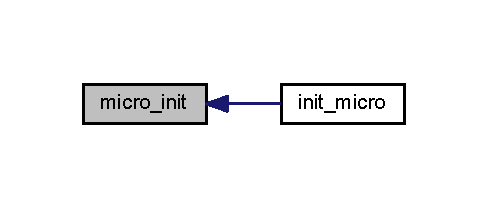
\includegraphics[width=234pt]{gsmddrive_8f_a545ecb105d9ac23b8913dfbf8655d0a0_icgraph}
\end{center}
\end{figure}



\hypertarget{mainpage_8txt}{}\section{zhang\+\_\+orig/mainpage.txt File Reference}
\label{mainpage_8txt}\index{zhang\+\_\+orig/mainpage.\+txt@{zhang\+\_\+orig/mainpage.\+txt}}

\hypertarget{precpd_8f}{}\section{precpd.\+f File Reference}
\label{precpd_8f}\index{precpd.\+f@{precpd.\+f}}
\subsection*{Functions/\+Subroutines}
\begin{DoxyCompactItemize}
\item 
subroutine \hyperlink{precpd_8f_ae4ad929ece53fb2262d73d3a614c0600}{precpd} (im, ix, km, dt, del, prsl, q, cwm, t, rn, sr                                           ,                                                                   rainp, u00k, psautco, prautco, evpco, wminco                       ,                                                                   lprnt, jpr)
\begin{DoxyCompactList}\small\item\em This subroutine is for precipitation processes from suspended cloud water/ice. \end{DoxyCompactList}\end{DoxyCompactItemize}


\subsection{Function/\+Subroutine Documentation}
\index{precpd.\+f@{precpd.\+f}!precpd@{precpd}}
\index{precpd@{precpd}!precpd.\+f@{precpd.\+f}}
\subsubsection[{\texorpdfstring{precpd(im, ix, km, dt, del, prsl, q, cwm, t, rn, sr                                           ,                                                                   rainp, u00k, psautco, prautco, evpco, wminco                       ,                                                                   lprnt, jpr)}{precpd(im, ix, km, dt, del, prsl, q, cwm, t, rn, sr                                           ,                                                                   rainp, u00k, psautco, prautco, evpco, wminco                       ,                                                                   lprnt, jpr)}}]{\setlength{\rightskip}{0pt plus 5cm}subroutine precpd (
\begin{DoxyParamCaption}
\item[{integer}]{im, }
\item[{integer}]{ix, }
\item[{integer}]{km, }
\item[{}]{dt, }
\item[{}]{del, }
\item[{}]{prsl, }
\item[{real (kind=kind\+\_\+phys), dimension(ix,km)}]{q, }
\item[{real (kind=kind\+\_\+phys), dimension(ix,km)}]{cwm, }
\item[{real (kind=kind\+\_\+phys), dimension(ix,km)}]{t, }
\item[{}]{rn, }
\item[{}]{sr, }
\item[{}]{rainp, }
\item[{}]{u00k, }
\item[{}]{psautco, }
\item[{}]{prautco, }
\item[{}]{evpco, }
\item[{}]{wminco, }
\item[{logical}]{lprnt, }
\item[{integer}]{jpr}
\end{DoxyParamCaption}
)}\hypertarget{precpd_8f_ae4ad929ece53fb2262d73d3a614c0600}{}\label{precpd_8f_ae4ad929ece53fb2262d73d3a614c0600}
\begin{DoxyRefDesc}{Todo}
\item[\hyperlink{todo__todo000002}{Todo}]param @\mbox{[} \end{DoxyRefDesc}

\begin{DoxyEnumerate}
\item Select columns where rain can be produced
\item Begining of precipitation calculation 
\end{DoxyEnumerate}

Definition at line 7 of file precpd.\+f.



Referenced by gbphys().



Here is the caller graph for this function\+:
\nopagebreak
\begin{figure}[H]
\begin{center}
\leavevmode
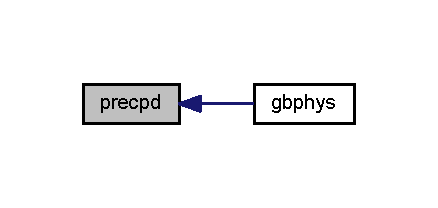
\includegraphics[width=210pt]{precpd_8f_ae4ad929ece53fb2262d73d3a614c0600_icgraph}
\end{center}
\end{figure}



\hypertarget{precpd__shoc_8f}{}\section{precpd\+\_\+shoc.\+f File Reference}
\label{precpd__shoc_8f}\index{precpd\+\_\+shoc.\+f@{precpd\+\_\+shoc.\+f}}
\subsection*{Functions/\+Subroutines}
\begin{DoxyCompactItemize}
\item 
subroutine \hyperlink{precpd__shoc_8f_a9dc8dede4aa2694932f96efe2fb29608}{precpd\+\_\+shoc} (im, ix, km, dt, del, prsl, q, cwm, t, rn, sr
\end{DoxyCompactItemize}


\subsection{Function/\+Subroutine Documentation}
\index{precpd\+\_\+shoc.\+f@{precpd\+\_\+shoc.\+f}!precpd\+\_\+shoc@{precpd\+\_\+shoc}}
\index{precpd\+\_\+shoc@{precpd\+\_\+shoc}!precpd\+\_\+shoc.\+f@{precpd\+\_\+shoc.\+f}}
\subsubsection[{\texorpdfstring{precpd\+\_\+shoc(im, ix, km, dt, del, prsl, q, cwm, t, rn, sr}{precpd_shoc(im, ix, km, dt, del, prsl, q, cwm, t, rn, sr}}]{\setlength{\rightskip}{0pt plus 5cm}subroutine precpd\+\_\+shoc (
\begin{DoxyParamCaption}
\item[{integer}]{im, }
\item[{integer}]{ix, }
\item[{integer}]{km, }
\item[{real (kind=kind\+\_\+phys)}]{dt, }
\item[{real (kind=kind\+\_\+phys), dimension(ix,km)}]{del, }
\item[{real (kind=kind\+\_\+phys), dimension(ix,km)}]{prsl, }
\item[{real (kind=kind\+\_\+phys), dimension(ix,km)}]{q, }
\item[{real (kind=kind\+\_\+phys), dimension(ix,km)}]{cwm, }
\item[{real (kind=kind\+\_\+phys), dimension(ix,km)}]{t, }
\item[{real (kind=kind\+\_\+phys), dimension(im)}]{rn, }
\item[{real (kind=kind\+\_\+phys), dimension(im)}]{sr}
\end{DoxyParamCaption}
)}\hypertarget{precpd__shoc_8f_a9dc8dede4aa2694932f96efe2fb29608}{}\label{precpd__shoc_8f_a9dc8dede4aa2694932f96efe2fb29608}


Definition at line 2 of file precpd\+\_\+shoc.\+f.



Referenced by gbphys().



Here is the caller graph for this function\+:\nopagebreak
\begin{figure}[H]
\begin{center}
\leavevmode
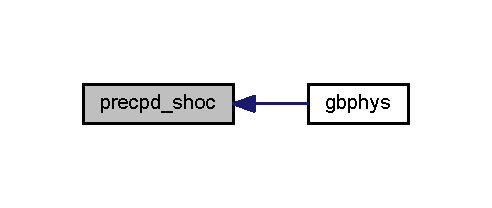
\includegraphics[width=236pt]{precpd__shoc_8f_a9dc8dede4aa2694932f96efe2fb29608_icgraph}
\end{center}
\end{figure}



\hypertarget{precpdp_8f}{}\section{precpdp.\+f File Reference}
\label{precpdp_8f}\index{precpdp.\+f@{precpdp.\+f}}
\subsection*{Functions/\+Subroutines}
\begin{DoxyCompactItemize}
\item 
subroutine \hyperlink{precpdp_8f_a6a36aa3f4d8cc8fb1b44aab270d3e625}{precpdp} (im, ix, km, dt, del, prsl, ps, q, cwm, t, rn, sr
\end{DoxyCompactItemize}


\subsection{Function/\+Subroutine Documentation}
\index{precpdp.\+f@{precpdp.\+f}!precpdp@{precpdp}}
\index{precpdp@{precpdp}!precpdp.\+f@{precpdp.\+f}}
\subsubsection[{\texorpdfstring{precpdp(im, ix, km, dt, del, prsl, ps, q, cwm, t, rn, sr}{precpdp(im, ix, km, dt, del, prsl, ps, q, cwm, t, rn, sr}}]{\setlength{\rightskip}{0pt plus 5cm}subroutine precpdp (
\begin{DoxyParamCaption}
\item[{integer}]{im, }
\item[{integer}]{ix, }
\item[{integer}]{km, }
\item[{}]{dt, }
\item[{}]{del, }
\item[{}]{prsl, }
\item[{}]{ps, }
\item[{real (kind=kind\+\_\+phys), dimension(ix,km)}]{q, }
\item[{real (kind=kind\+\_\+phys), dimension(ix,km)}]{cwm, }
\item[{real (kind=kind\+\_\+phys), dimension(ix,km)}]{t, }
\item[{}]{rn, }
\item[{}]{sr}
\end{DoxyParamCaption}
)}\hypertarget{precpdp_8f_a6a36aa3f4d8cc8fb1b44aab270d3e625}{}\label{precpdp_8f_a6a36aa3f4d8cc8fb1b44aab270d3e625}


Definition at line 2 of file precpdp.\+f.



Referenced by gbphys().



Here is the caller graph for this function\+:
\nopagebreak
\begin{figure}[H]
\begin{center}
\leavevmode
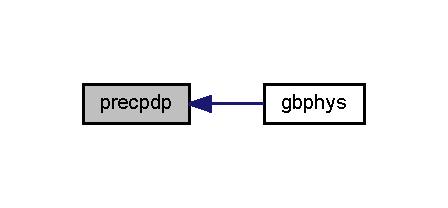
\includegraphics[width=215pt]{precpdp_8f_a6a36aa3f4d8cc8fb1b44aab270d3e625_icgraph}
\end{center}
\end{figure}



%--- End generated contents ---

% Index
\backmatter
\newpage
\phantomsection
\clearemptydoublepage
\addcontentsline{toc}{chapter}{Index}
\printindex

\end{document}
